\subsection{Meldeprint}
Die Software des Meldeprints ist in drei Bereiche unterteilt: Initialisierung, Interrupt, Statusüberwachung. Beinahe die ganze Überwachung der Module kann im Bereich Statusüberwachung abgehandelt werden. Die anderen beiden dienen zum einen für die Anzeige und die Initialisierung und zum anderen für die Aktualisierung der eingehenden Daten.

\begin{figure}[htbp] 
  \centering
     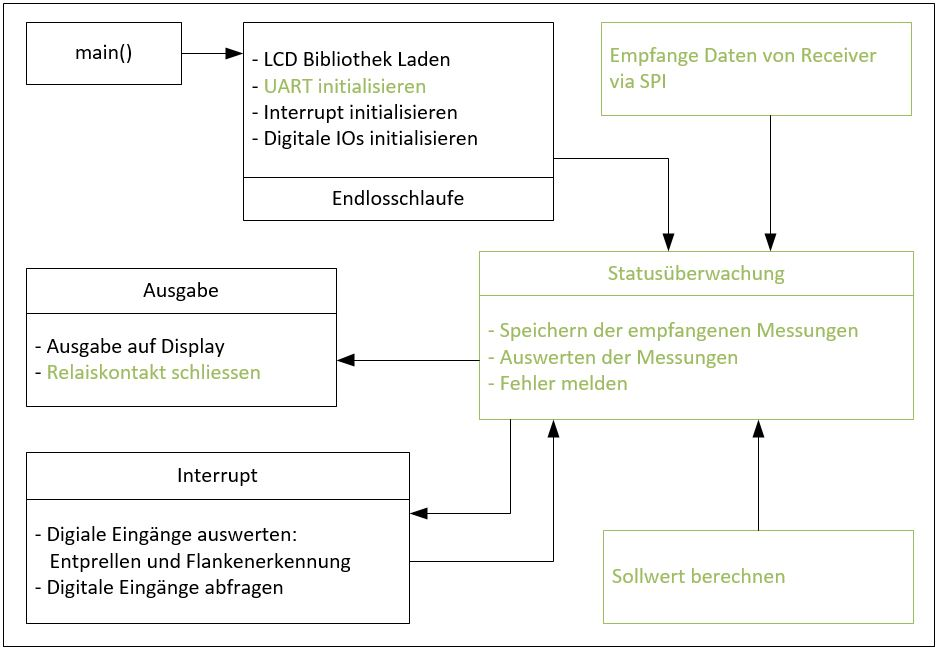
\includegraphics[width=1\textwidth]{graphics/reportboard-software-river}
  \caption{Visualisierung Softwarekonzept}
  \label{fig:reportboard-software-river}
\end{figure}

Wie die Bereiche der Software zusammenarbeiten ist in Abbildung \ref{fig:reportboard-software-river} gut ersichtlich. In der Initialisierung wird als Erstes die Hardwarekomponenten und Interrupts initialisiert, dann wird die Endlosschlaufe im Hauptprogramm aufgerufen.\\
Der Timer-Interrupt ruft dann alle 15$\mu$s die Input-Routine auf, die digitale Eingänge entprellt und eine Flankendetektion durchführt. Eingehende und an das Hauptprogramm übermittelte Daten vom Receiver lösen einen Interrupt aus, der die Datenpakete weiterverarbeitet.\\
Die Endlosschlaufe ruft die Prozess-Routine auf, die jeweils eingegangene Daten, der gemessenen Spannung, mit der Identifikationsnummer des Sensorprints in ein Array speichert und mit dem Sollwert vergleicht. Der Sollwert entspricht dem arithmetischen Mittelwert der Spannungen dieses einen Strings von Modulen. Bei einer Abweichung von 20 Prozent\todo{sind diese 20 Prozent endgültig?} wird dasjenige Modul vorgemerkt. Falls nach einer weiteren Messung die Spannung desselben Moduls gleichviel vom Mittelwert abweicht, muss ein Fehler gemeldet werden. Die Identifikationsnummer wird auf dem Display angezeigt. Der ganze Prozess vom Start des Meldeprints bis zur Fehlermeldung werden hier weiter vertieft behandelt. Dabei ist anzumerken, dass die ganzen hier beschriebenen Prozesse nicht abschliessend programmiert und getestet werden konnten. Es lag wohl an der zu grossen Wissenslücke im Standard C Programmieren.

\subsubsection{Inbetriebnahme}
Wird die Hardware mit Energie versorgt, startet die Software des Meldeprints und initialisiert als erstes die Peripheriegeräte. Darunter befinden sich der LCD-Display und der Receiver. Weiter muss die UART-Kommunikation, der normale und der Timer-Interrupt initialisiert werden. Ist dieser Vorgang abgeschlossen ruft die Endlosschlaufe im Hauptprogramm die berechnende Routine auf für die Fehlererkennung des Sensorprints. Der Meldeprint ist nun betriebsbereit und reagiert sobald eine Eingabe vom Benutzer getätigt wird oder der Interrupt ein eingehendes Datenpaket registriert. Die Datenpakete des Sensorprints würden nun erkannt und im Hauptprogramm in ein Registerarray gespeichert.

\subsubsection{Receiver}
Der Receiver detektiert über einen Ferrit-Kern über der DC-Leitung des Strings die Signale des Sensorprints. Die Datenpakete werden mit der Identifikationsnummer zuerst über die UART Kommunikation an den Arduino weitergeleitet.\\
Die Kommunikation über die DC-Leitung zwischen Sensorprint und Meldeprint ist Unidirektional. Ist der Meldeprint eingeschaltet und die Initialisierung des Receivers abgeschlossen, können laufend vom Sensorprint gesendete Datenpakete empfangen werden. Der im Hauptprogramm zuvor initialisierte Interrupt registriert die empfangenen Daten vom Receiver und verarbeitet diese weiter.

\subsubsection{Fehlererkennung}
Die Fehlererkennung spielt eine wichtige Rolle im gesamten Überwachungssystem von Sensor- und Meldeprint. Es gab mehrere diskutierte Varianten, wie nun ein Fehler eines einzelnen Moduls gefunden und lokalisiert werden konnte. Als übersichtlichste und beste Variante diente sich das arithmetische Mittel mit einer Identifikationsnummer an.

\begin{figure}[htbp] 
  \centering
     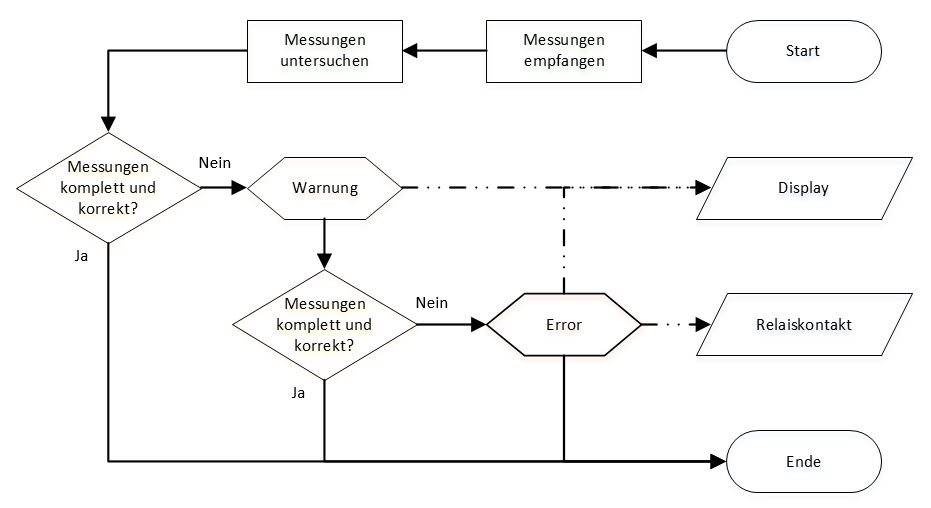
\includegraphics[width=1\textwidth]{graphics/error-warning-scheme}
  \caption{Prozess zur Fehlererkennung}
  \label{fig:error-warning-scheme}
\end{figure}

\begin{figure}[htbp] 
  \centering
     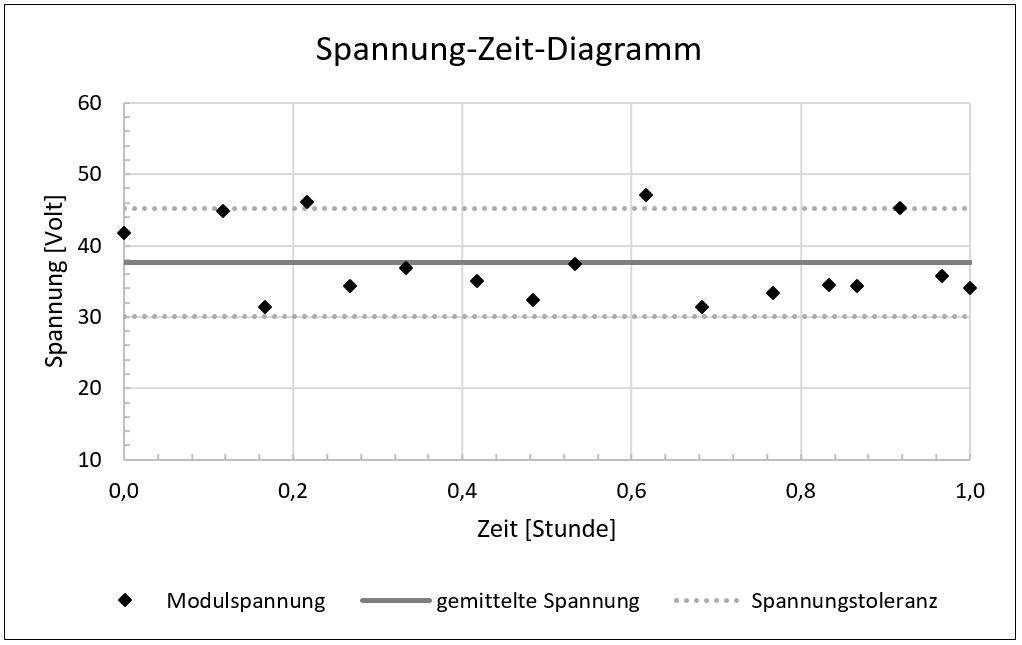
\includegraphics[width=1\textwidth]{graphics/failurecalc-diagram}
  \caption{Spannung-Zeit-Diagramm: Alle übermittelten Modulspannungen innerhalb einer Stunde}
  \label{fig:failurecalc-diagram}
\end{figure}

Die Variante will die gemittelten Spannungswerte, die jede Sensorplatine liefert, nochmals über alle Module des Strings mitteln. Damit kann die Standardabweichung berechnet werden.\todo{Haben wir eine Rechnung für Standardabweichung} Ist die Abweichung eines Wertes mehr als 20 Prozent über der Standardabweichung, wird dieses Solarmodul vorgemerkt. Weicht der Spannungswert des vorgemerkten Moduls nach der nächsten Stunde noch immer stark vom Mittelwert ab, wird eine Fehlermeldung ausgegeben. Eine dem fehlerbehafteten Mittelwert hinterlegte Identifikationsnummer erlaubt es das Modul exakt zu nennen und es im überwachten String zu finden. Dieser Prozess wiederholt sich stündlich und ist in Abbildung \ref{fig:error-warning-scheme} sichtbar, weiter zeigt die Abbildung \ref{fig:failurecalc-diagram} die übermittelten Modulspannungen und solche, die eine zu grosse Toleranz haben und deshalb vorgemerkt werden.

\subsubsection{Fehlermeldung (Display und Relais)}
Die Fehlermeldung besteht aus der Fehlerankündigung selbst und der Identifikationsnummer der Sensorplatine, welche am überwachten Modul befestigt ist. Die Fehlerankündigung ist als Text wie beispielsweise "Problem bei Modul..." auf dem Display zu sehen. Die Identifikationsnummer des Moduls wird von einer 8bit Binärzahl in eine Dezimalzahl umgewandelt und so angezeigt.

\subsubsection{Benutzerinterface (Display und Drehgeber)}
Das Menü und der Drehgeber bilden zusammen eine einfache Schnittstelle zwischen Mensch und Maschine. Das Menü ist in zwei Ebenen unterteilt welche in Abbildung \ref{fig:structure-menu} dargestellt ist.

\begin{figure}[htbp] 
  \centering
     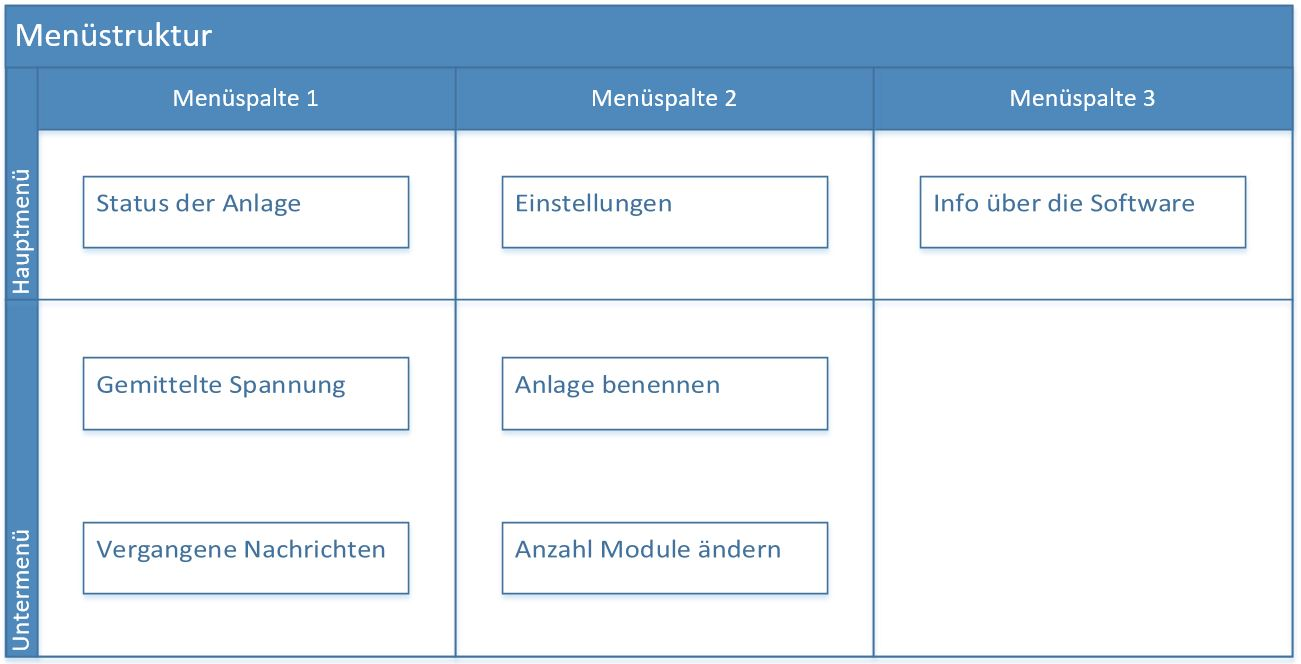
\includegraphics[width=1\textwidth]{graphics/structure-menu}
  \caption{Menüstruktur}
  \label{fig:structure-menu}
\end{figure}

In der Hauptmenü-Zeile befinden sich die drei Einträge: "Status der Anlage", "Einstellungen" und "Info über die Software". In der Untermenü-Zeile kann der Benutzer in der ersten Menüspalte zum Ersten die aktuell gemittelte Spannung abfragen, zum Zweiten die erechnete Leistung der Anlage abfragen und zum Dritten alle Nachrichten seit dem letzten Zurücksetzen des Meldeprints nachschauen. In der zweiten Menüspalte kann der Benutzer Einstellungen vornehmen. Das sind zum einen der Anlage einen Namen geben, falls diese, vom Meldeprint überwachten, Strings ein Teil einer grösseren Anlage sind. Zum Anderen muss die Menge der überwachten Module angegeben werden für die Speicherung, Identifikation und Überwachung. In der dritten Menüspalte werden Informationen zur aktuellen Software und dem Hersteller angezeigt. Um in eine Menüspalte oder einen Untermenü-Eintrag zu gelangen wird der Drehgeber gedrückt zudem ist in jeder Menüspalte und jedem Untermenü-Eintrag eine Zurück-Funktion, um wieder auf die nächst höhere Ebene zu gelangen.